\section{Point--Line Incidences}

The crossing lemma also bounds how often points of the plane can lie on lines, and the bound in turn says something about sums and products of integers.

\subsection{The Szemer\'{e}di--Trotter Theorem}

Given finite sets $\mathcal{L}$ of lines and $P$ of points in $\R^2$, define
\begin{align*}
    I\of{\mathcal{L}, P}
    := \#\!\set{\text{point-line incidences}}
    = \#\!\setst{\parenth{\ell, p} \in \mathcal{L} \times P}{p \in \ell}
\end{align*}

It turns out that we can say how large this can be, up to a constant.

\begin{boxtheorem}[Szemer\'{e}di--Trotter] \label{Ch7:Thm:Szemeredi_Trotter}
    $I\of{\mathcal{L}, P} = \BigO{\abs{\mathcal{L}}^{\frac{2}{3}} \abs{P}^{\frac{2}{3}} + \abs{\mathcal{L}} + \abs{P}}$
\end{boxtheorem}
\begin{proof}
    Given an $\mathcal{L},P$ system, consider the graph drawing $D$ whose vertices are the points in $P$ and whose edges are intervals of lines in $\mathcal{L}$ with endpoints in $P$, with no interior points in $P$.

    % [CORRECTED] was: "Let $P'$ with $\abs{P'} \leq \abs{P} + 2 \abs{\mathcal{L}}$ be an expected set of points such that every line has $\geq 2$ points." --- with up to $2\abs{\mathcal{L}}$ added points the argument below gives a term of order $\abs{\mathcal{L}}^{4/3}$, which the bound cannot absorb when $\abs{\mathcal{L}}$ is much larger than $\abs{P}$. The sentence now carries out the reduction of the author's own comment, which stood here: "I need to assume here that each line has at least 2 points. Then I argue and get my bound. Now in the general case, what I do is, I remove all lines with just one point, I get my upper-bound, then I add them back, which adds at most |L|, which gets subsumed into the |L| term of our big O."
    We first assume that every line of $\mathcal{L}$ contains at least $2$ points of $P$. In the general case, we remove the lines containing fewer than $2$ points of $P$, get our upper-bound for the lines that remain, and then add them back, which adds at most $\abs{\mathcal{L}}$ incidences; these are absorbed into the $\abs{\mathcal{L}}$ term of the bound.

    Let $n = \abs{P}$ be the number of vertices. How many edges do I have? I should have
    \begin{align*}
        m
        = I\of{\mathcal{L}, P} - \abs{\mathcal{L}}
        = \sum_{\ell \in \mathcal{L}} \parenth{\#\!\setst{p \in P}{p \in \ell} - 1}
    \end{align*}
    % [CORRECTED] was: "$n \leq 4m$, ie, $\abs{P'} \leq 4\parenth{I\of{\mathcal{L}, P} - \abs{P}}$" --- the crossing lemma needs $m \geq 4n$, and $m = I\of{\mathcal{L}, P} - \abs{\mathcal{L}}$
    If we have $4n \leq m$, ie,
    \begin{align*}
        4\abs{P} \leq I\of{\mathcal{L}, P} - \abs{\mathcal{L}}
    \end{align*}
    % [CORRECTED] was: "$\pcr{D} \leq \frac{\parenth{I\of{\mathcal{L}, P} - \abs{P}}^3}{64 \abs{P'}^2}$" --- the crossing lemma bounds $\pcr{D}$ from below, by $\frac{m^3}{64n^2}$
    then we can apply \Cref{Ch7:Thm:Crossing_Lemma} to conclude that
    \begin{align*}
        \pcr{D} \geq \frac{\parenth{I\of{\mathcal{L}, P} - \abs{\mathcal{L}}}^3}{64 \abs{P}^2}
    \end{align*}
    \sorry
    % Hint (from the blackboard): bound $\pcr{D}$ from above by $\abs{\mathcal{L}}^2$ --- where can two edges of $D$ cross, and how often can two lines meet? Comparing the two bounds on $\pcr{D}$ bounds $m$, and so $I\of{\mathcal{L}, P}$; the case $m < 4n$ needs a line of its own.
\end{proof}

\subsection{Sums and Products}

Fix some $A \ssq \Z$. Define
\begin{align*}
    A + A &:= \setst{a + b}{a, b \in A} \\
    A \cdot A &:= \setst{a \cdot b}{a, b \in A}
\end{align*}

Is there a set $A$ for which both $A + A$ and $A \cdot A$ are small?

To answer this, we turn it into an incidence problem. Define
\begin{align*}
    P := \parenth{A + A} \times \parenth{A \cdot A}
    = \setst{(x, y) \in \Z \times \Z}{x \in A + A, \, y \in A \cdot A}
\end{align*}
For example, when $A = \set{1, 2, 3}$, we have $A + A = \set{2, \ldots, 6}$ and $A \cdot A = \set{1, 2, 3, 4, 6, 9}$, and $P$ looks like this.
\begin{figure}[H]
    \centering
    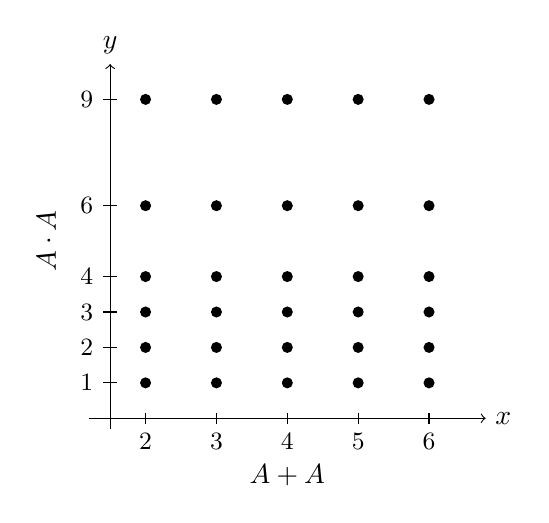
\begin{tikzpicture}[x = 0.9cm, y = 0.45cm]
        \draw[->] (1.2, 0) -- (6.8, 0) node[right] {$x$};
        \draw[->] (1.5, -0.3) -- (1.5, 10) node[above] {$y$};
        \foreach \x in {2, ..., 6}{
            \draw (\x, 0.15) -- (\x, -0.15) node[below] {\small $\x$};
        }
        \foreach \y in {1, 2, 3, 4, 6, 9}{
            \draw (1.6, \y) -- (1.4, \y) node[left] {\small $\y$};
            \foreach \x in {2, ..., 6}{
                \fill[black] (\x, \y) circle (2pt);
            }
        }
        \node at (4, -1.6) {$A + A$};
        \node[rotate = 90] at (0.6, 5) {$A \cdot A$};
    \end{tikzpicture}
\end{figure}

The incidence bound answers our question: $A + A$ and $A \cdot A$ cannot both be small.

% [FILLED] statement written up from the blackboard photographs supplied on 2026-10-27; the proof is left to the author, with a hint
\begin{boxtheorem} \label{Ch7:Thm:Sum_Product}
    There is a constant $c > 0$ such that for every finite $A \ssq \Z$,
    \begin{align*}
        \abs{A + A} \abs{A \cdot A} \geq c \abs{A}^{\frac{5}{2}}
    \end{align*}
    In particular, $\max\set{\abs{A + A}, \abs{A \cdot A}} \geq \sqrt{c} \abs{A}^{\frac{5}{4}}$.
\end{boxtheorem}
\begin{proof}
    \sorry
    % Hint (from the blackboard): use $P$ as above, so that $\abs{P} = \abs{A + A}\abs{A \cdot A}$, and let $\mathcal{L}$ be the $\abs{A}^2$ lines $y = a\parenth{x - a'}$ for $a, a' \in A$ (assume $0 \notin A$). Each of them passes through $\abs{A}$ points of $P$ --- try $x = a' + b$ for $b \in A$ --- so $I\of{\mathcal{L}, P} \geq \abs{A}^3$. Now compare this with \Cref{Ch7:Thm:Szemeredi_Trotter}, one term of its bound at a time.
\end{proof}
